\documentclass[oneside, final, 12pt]{article}

\pagestyle{plain}

\usepackage{a4wide}
\usepackage[utf8]{inputenc}
\usepackage[russian]{babel}
\usepackage{vmargin}
\setpapersize{A4}
\setmarginsrb{2cm}{1.5cm}{1cm}{1.5cm}{5pt}{5mm}{5pt}{13mm}
\usepackage{indentfirst}
\usepackage{graphicx}

\usepackage{amsmath}
\usepackage{amsfonts}
\usepackage{amsthm}
\usepackage{amssymb}

\newcommand{\norm}[1]{\left\lVert #1 \right\rVert}

\newtheorem{definition}{Определение}
\newtheorem{feature}{Свойство}
\newtheorem{statement}{Утверждение}
\newtheorem{sthm}{Теорема}


\begin{document}


\thispagestyle{empty}

\begin{center}
\ \vspace{-3cm}


\includegraphics[width=0.5\textwidth]{msu.eps}\\
{\scshape Московский государственный университет имени М.~В.~Ломоносова}\\
Факультет вычислительной математики и кибернетики\\
Кафедра системного анализа

\vfill

\begin{LARGE}
	Отчёт по практикуму

\end{LARGE}

\vspace{1cm}

\begin{Huge}
\bfseries <<Прикладные задачи системного анализа: задачи биоматематики>>

\end{Huge}

\end{center}

\vspace{1cm}

\begin{flushright}
  \large
  \textit{Студентка 515 группы}\\
  А.\,А.~Наумова

  \vspace{5mm}

  \textit{Руководитель практикума}\\
   аспирант Д.\,А.~Алимов

\end{flushright}

\vfill

\begin{center}
Москва, 2020
\end{center}

\newpage
\tableofcontents								%	СОДЕРЖАНИЕ

\newpage
\section{Постановка задачи}						%	ПОСТАНОВКА ЗАДАЧИ
Дана система, описывающая динамику численности популяций жертвы и хищника:
	\[
	\begin{cases}
	\dot{u} = au - \dfrac{bu^2v}{1 + Pu} + d_1u_{xx}, \\
	\dot{v} = -cv + \dfrac{du^2v}{1 + Pu} + d_2v_{xx}.
	\end{cases}
	\]

Требуется:
\begin{enumerate}
    \item Сделать замены переменных
    \item Исследовать фазовый портрет нераспределенной системы (неподвижные точки, их тип, изоклины)
    \item Проверить наличие волновых решений распределенной системы
    \item Выбрать подходящее решение и скорость волны
    \item Привести иллюстрации и графики фазовых портретов и решений
\end{enumerate}

\newpage
\section{Исследование нераспределенной системы}						%
\subsection{Замена переменных}
Пусть
\[
    \widetilde{u} = \alpha u;\\
    \widetilde{v} = \beta u;\\
    \widetilde{t} = \gamma t;\\
    \widetilde{x} = \delta x.
\]
Тогда система примет следующий вид:
\[
    \begin{cases}
        \dfrac{\gamma}{\alpha} \widetilde{u}_{\widetilde{t}} =
        \dfrac{a}{\alpha}\widetilde{u}
        - \dfrac{b}{\alpha^2\beta} \dfrac{\widetilde{u}^2\widetilde{v}}{(1 + P\widetilde{u}/\alpha)}
        + d_1\dfrac{\delta^2}{\alpha} \widetilde{u}_{\widetilde{x}\widetilde{x}}, \\

        \dfrac{\gamma}{\beta} \widetilde{v}_{\widetilde{t}} =
        \dfrac{-c}{\beta}\widetilde{v}
        + \dfrac{d}{\alpha^2\beta} \dfrac{\widetilde{u}^2\widetilde{v}}{(1 + P\widetilde{u}/\alpha)}
        + d_2\dfrac{\delta^2}{\beta} \widetilde{v}_{\widetilde{x}\widetilde{x}}.
    \end{cases}
\]
Чтобы избавиться от лишних коэффициентов, возьмем
\[
    \gamma = a;\\
    \beta = \dfrac{b}{a};\\
    \alpha = P;\\
    \delta = \sqrt{\dfrac{a}{d_2}}.
\]
Получим
\[
    \begin{cases}
        \dot{u} = u\left(1 - \dfrac{1}{P} \dfrac{uv}{1 + u}\right)  + \dfrac{d_1}{d_2}u_{xx}, \\
        \dot{v} = \dfrac{-c}{a} v\left(1 - \dfrac{d}{P^{2}c} \dfrac{u^2}{1 + u}\right) + v_{xx}.
    \end{cases}
\]
Переобозначим
\[
    k_1 = \dfrac{1}{P};\\
    k_2 = \dfrac{-c}{a};\\
    k_3 = \dfrac{d}{P^{2}c}.
\]
Предполагаем, что \(d_1 = 0\) (жертвы сконцентрированы в одной точке). Тогда получаем систему размерности 3:
\[
    \begin{cases}
        \dot{u} = u\left(1 -  k_1\dfrac{uv}{1 + u}\right) , \\
        \dot{v} = k_2 v\left(1 - k_3 \dfrac{u^2}{1 + u}\right) + v_{xx}.
    \end{cases}
\]

\subsection{Неподвижные точки и их тип}

Якобиан системы имеет вид:\\
J(u,v) =
\begin{pmatrix}
    \(1-k_1 uv\dfrac{2+u}{(1+u)^2}\) & \(-k_1 \dfrac{u^2}{1+u}\)\\
    \(-k_2 k_3 uv\dfrac{2 + u}{\left( 1+u \right)^2} \) & \(k_2 \left( 1 - k_3\dfrac{u^2}{1+u} \right)\)
\end{pmatrix}\\

Рассмотрим неподвижную точку \( T_1 = (0, 0).\) \\

Якобиан в этой точке принимает вид:
J(0,0) =
\begin{pmatrix}
    1 & 0\\
    0 & k_2
\end{pmatrix}\\

Так как существует собственное значение с положительной вещественной частью (\lambda_1=1\),
то данная точка неустойчива по теореме Ляпунова о неустойчивости по первому приближению.\\

Далее рассмотрим систему уравнений, решения которой отвечают изоклинам рассматриваемой системы:
\[
    \begin{cases}
        1 -  k_1\dfrac{uv}{1 + u} = 0, \\
        1 - k_3 \dfrac{u^2}{1 + u} = 0.
    \end{cases}
\]\\

Решение второго уравнения: \(u = \dfrac{1 \pm \sqrt{1+4k_3}}{2k_3} \).\\

Так как \(k_3 > 0\), в область \(\cal{R}^+\) попадает только \(u^* = \dfrac{1 + \sqrt{1+4k_3}}{2k_3} \).\\

Для удобства вычислений возьмем \(k_3 = 1 \). Также будем помнить, что \( k_1 > 0; k_2 \leq 0;\) (плюс еще надо не забыть рассмотреть случаи \(P=0; c=0; d=0\)).\\

Тогда \(u^* = \dfrac{1 + \sqrt{5}}{2}, v^* = \dfrac{1+u^*}{k_1 u^*} = \dfrac{1}{k_1} \left( 1 + \dfrac{2k_3}{1 + \sqrt{1+4k_3}} \right) = \dfrac{1}{k_1} \left( 1 + \dfrac{2}{1 + \sqrt{5}} \right) \).\\

Исследуем теперь данную неподвижную точку \( T_2 = (u^*, v^*).\) \\


Якобиан в этой точке принимает вид:\\

J(u*,v*) =
\begin{pmatrix}
    \(- \frac{\frac{\sqrt{5}}{2} + \frac{5}{2}}{\frac{\sqrt{5}}{2} + \frac{3}{2}} + 1\) & \(- \frac{k_{1} \left(\frac{1}{2} + \frac{\sqrt{5}}{2}\right)^{2}}{\frac{\sqrt{5}}{2} + \frac{3}{2}}\) \\
    \(- \frac{k_{2} \left(1 + \sqrt{5} + \left(\frac{1}{2} + \frac{\sqrt{5}}{2}\right)^{2}\right)}{k_{1} \left(\frac{1}{2} + \frac{\sqrt{5}}{2}\right) \left(\frac{\sqrt{5}}{2} + \frac{3}{2}\right)}\) & \(k_{2} \left(- \frac{\left(\frac{1}{2} + \frac{\sqrt{5}}{2}\right)^{2}}{\frac{\sqrt{5}}{2} + \frac{3}{2}} + 1\right)\)
\end{pmatrix}
\\

\(
\lambda_1 = - \frac{21 \sqrt{5} \sqrt{2728 \sqrt{5} k_{2} + 6100 k_{2} + 72 \sqrt{5} + 161}}{4} + \frac{47 \sqrt{2728 \sqrt{5} k_{2} + 6100 k_{2} + 72 \sqrt{5} + 161}}{4} - \frac{3}{4} + \frac{\sqrt{5}}{4}

\)\\

\(
\lambda_2 = - \frac{47 \sqrt{2728 \sqrt{5} k_{2} + 6100 k_{2} + 72 \sqrt{5} + 161}}{4} + \frac{21 \sqrt{5} \sqrt{2728 \sqrt{5} k_{2} + 6100 k_{2} + 72 \sqrt{5} + 161}}{4} - \frac{3}{4} + \frac{\sqrt{5}}{4}

\)\\

После упрощения выражений и численного вычисления значений получаем:\\

\(
\lambda_1 = - 0.190983005625053 + 1.17557050458504\sqrt{(k_2 + 0.026393202250021)}
\)\\

\(
\lambda_2 = - 0.190983005625053 - 1.17557050458504\sqrt{(k_2 + 0.026393202250021)}
\)\\

Заметим, что при \(k_2 = (\dfrac{0.190983005625053 }{1.17557050458504})^2 - 0.026393202250021 = 0  \)  \(\lambda_1 = 0\). Вспомним также, что \(k_2 \leq 0\).  Получим несколько возможных случаев.\\

1) \( -0.026393202250021 \leq k_2 < 0\).\\

\(
\lambda_1, \lambda_2 < 0
\)\\

2) \(k_2 < -0.026393202250021 \).\\

\( Re(\lambda_1)<0, Re(\lambda_2)<0, Im(\lambda_1)>0, Im(\lambda_2)<0 \)\\

Оба положения устойчивы.\\

\subsection{Фазовый портрет}

\subsubsection{Случай 1}
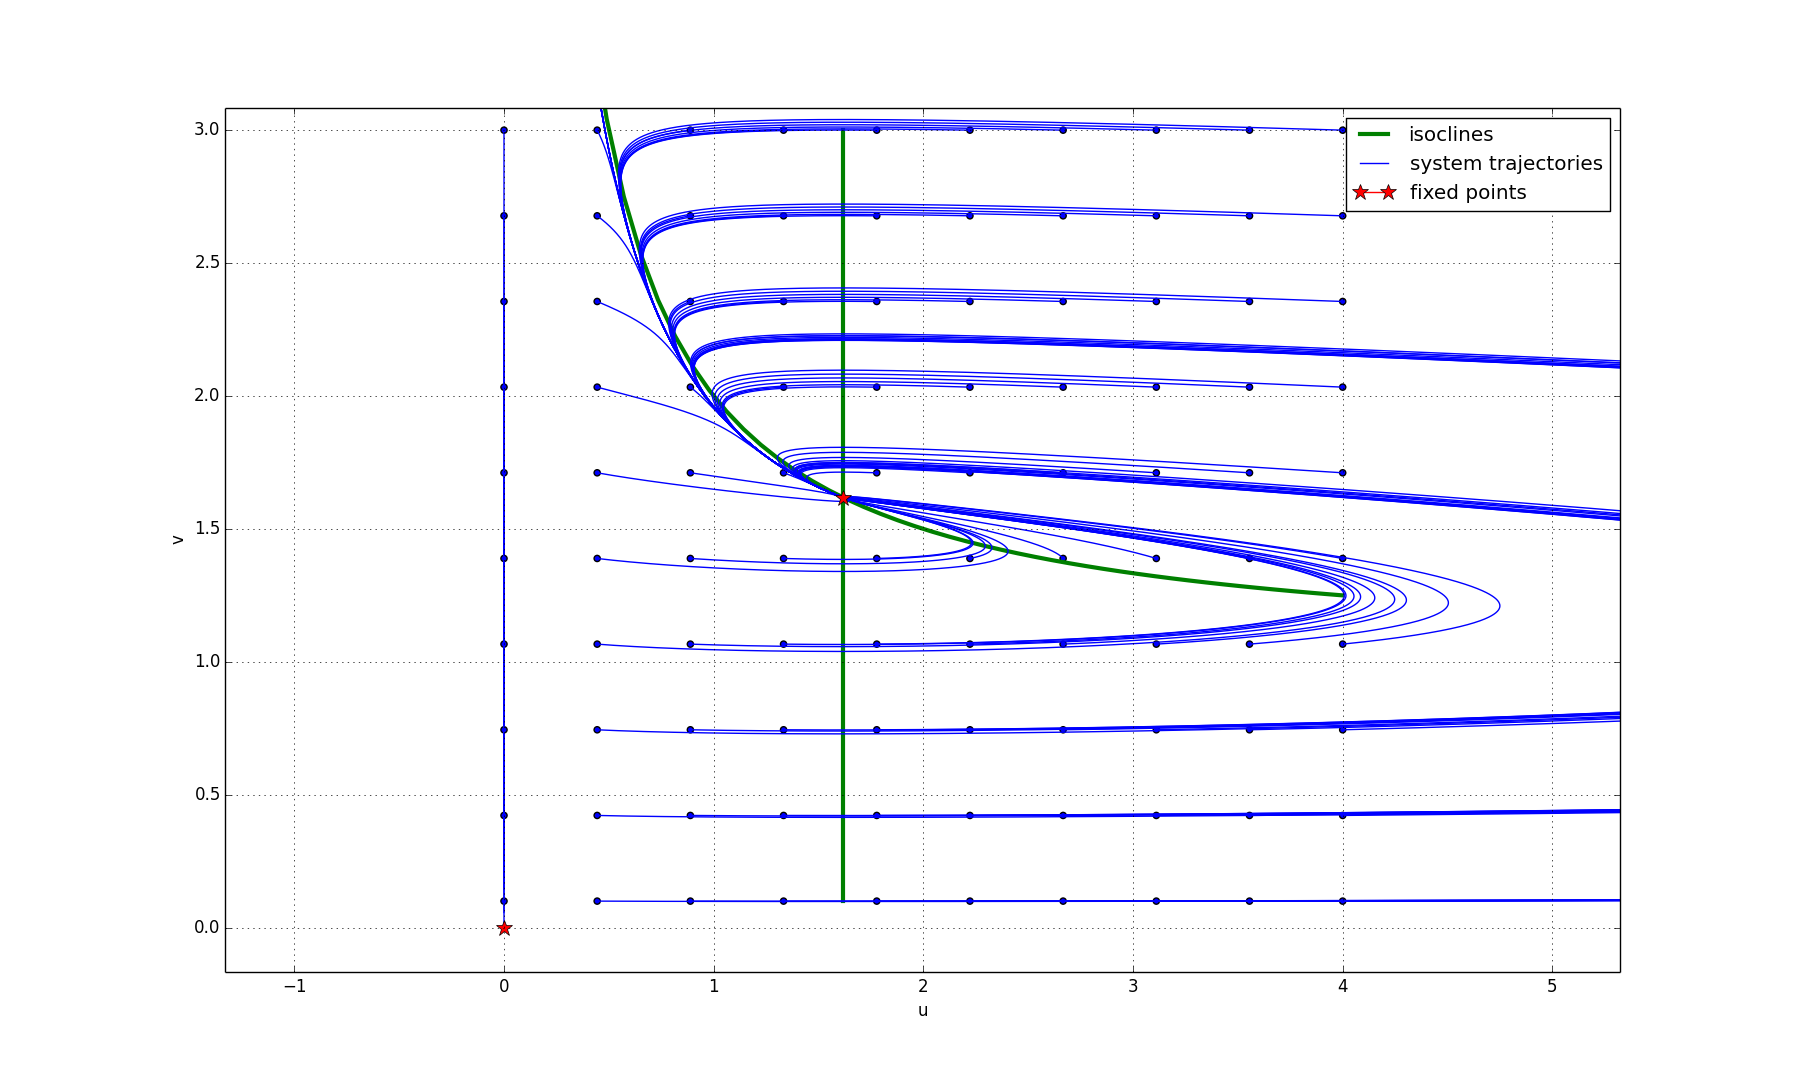
\includegraphics[width=1\textwidth]{figure_2.png}\\
Данный фазовый портрет был построен при \(k_1 = 1,k_2 = -0.02,k_3 = 1\), точки начала траекторий расположены на сетке 10х10, с параметрами start_u = 0.0, stop_u = 4.0, start_v = 0.1, stop_v = 3.0, stop_t = 100, num_t = 10000.\\

Видим, что неподвижная точка \( T_2 = (u^*, v^*)\) устойчива, к ней устремляются все трактории, кроме наинающихся в 0. А точка \( T_1 = (0,0)\) неучтойчива - траектории с \(u_0 = 0\) стремятся к ней, а траектории с \(v_0 = 0\) удаляются от нее.

\subsubsection{Случай 2}
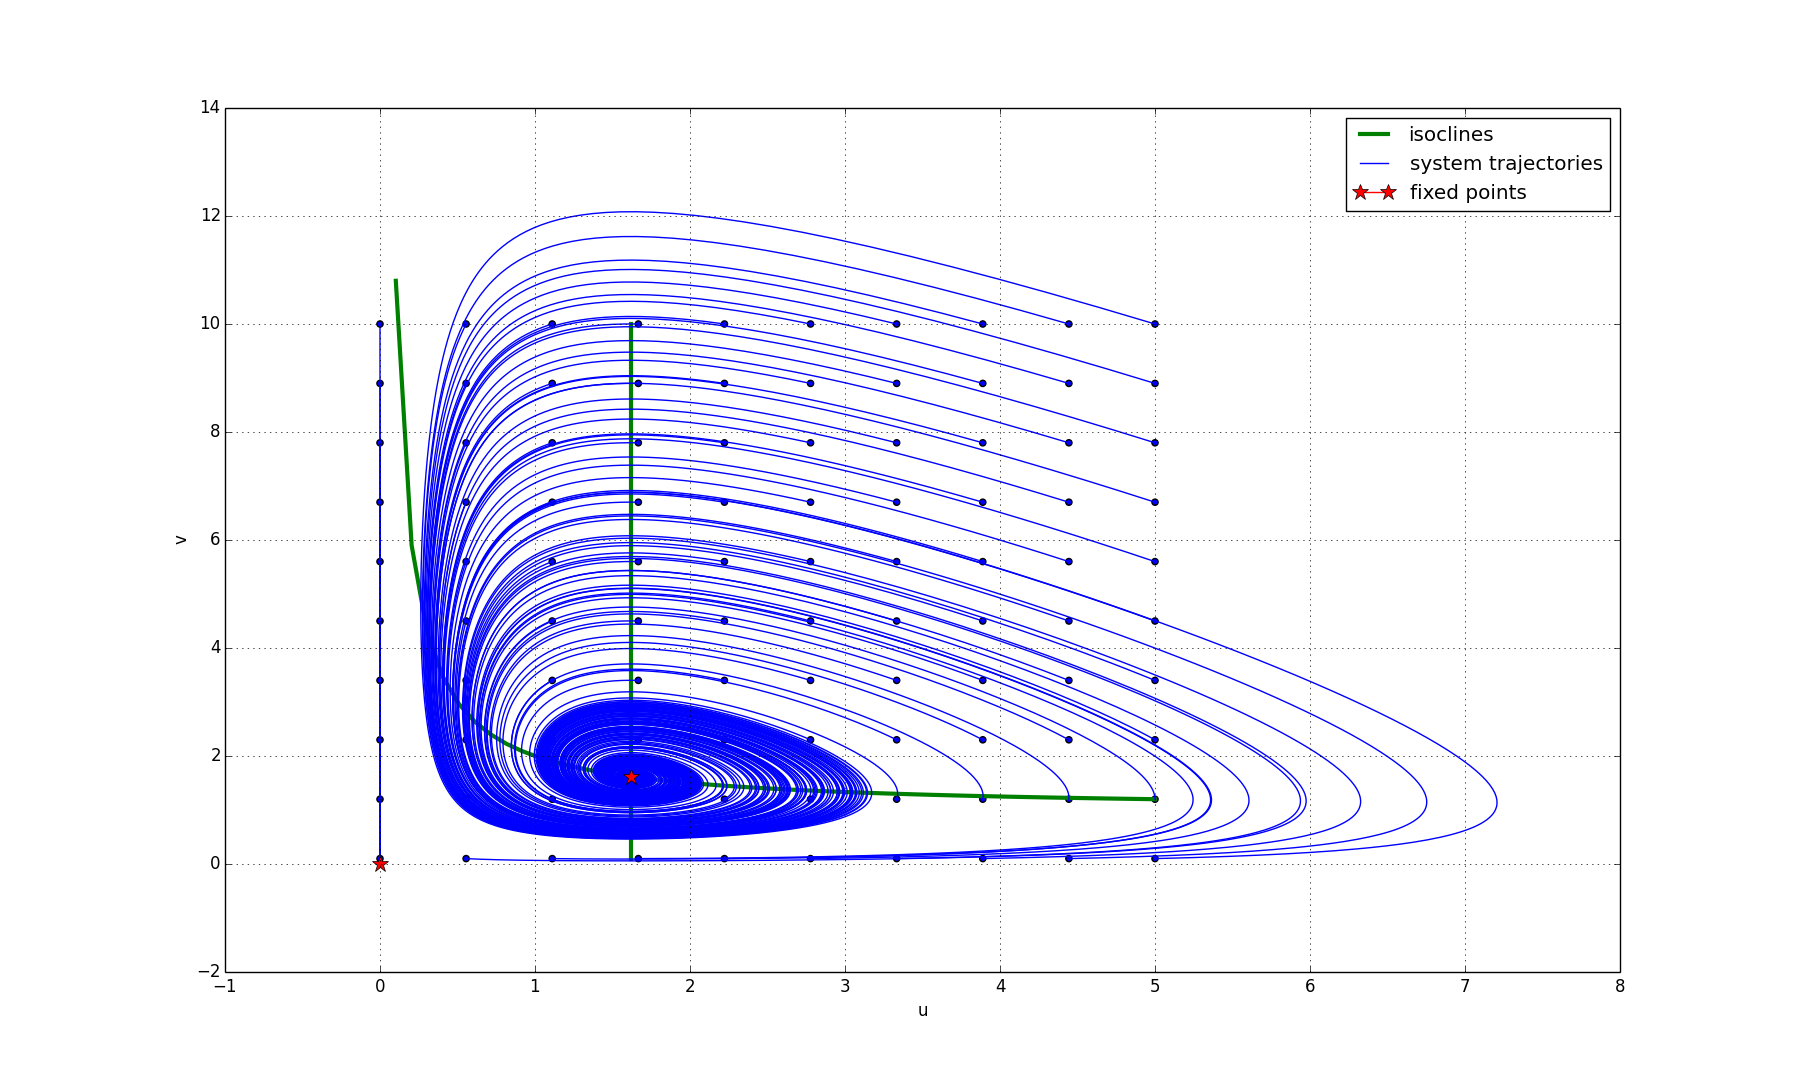
\includegraphics[width=1\textwidth]{figure_1.png}\\
Данный фазовый портрет был построен при \(k_1 = 1,k_2 = -1,k_3 = 1\), точки начала траекторий расположены на сетке 10х10, с параметрами start_u = 0.0, stop_u = 5.0, start_v = 0.1, stop_v = 10.0, stop_t = 100, num_t = 10000.\\



\newpage
\section{Исследование распределенной системы}
\subsection{Замена переменных}
Волновые решения ищем в форме:  \(u(t,x)=u(x+ct), v(t,x)=v(x+ct) \), где \(c>0\). Подставим это в уравнение системы. Получим:\\
\[
    \begin{cases}
        c u^\prime(z) = u(z)\left(1 -  k_1\dfrac{u(z)v(z)}{1 + u(z)}\right) , \\
        c v^\prime(z) = k_2 v(z)\left(1 - k_3 \dfrac{u(z)^2}{1 + u(z)}\right) + v^{\prime\prime}(z).
    \end{cases}
\]

Введем переменную w и перепишем систему:\\
\[
    \begin{cases}
        c u^\prime(z) = u(z)\left(1 -  k_1\dfrac{u(z)v(z)}{1 + u(z)}\right) , \\
        v^\prime(z) = w(z) , \\
        w^\prime(z) = cw(z) - k_2 v(z)\left(1 - k_3 \dfrac{u(z)^2}{1 + u(z)}\right).
    \end{cases}
\]

\subsection{Неподвижные точки и их тип}
У этой системы 2 неподвижных точки, попадающих в рассматриваемую область значений:
\(\overline{O} = (0, 0, 0)\) и \(\overline{P} = (u^*,v^*,0)\), где \(u^* = \dfrac{1 + \sqrt{5}}{2}, v^* = \dfrac{1}{k_1} \left( 1 + \dfrac{2}{1 + \sqrt{5}} \right) \).\\

Якобиан системы имеет вид:\\
J(u,v,w) =
\begin{pmatrix}
    \(\dfrac{1}{c} (1-k_1 uv\dfrac{2+u}{(1+u)^2})\) & \(\dfrac{-k_1}{c} \dfrac{u^2}{1+u}\) & 0\\
    0 & 0 & 1 \\
    \(k_2 k_3 uv\dfrac{2 + u}{\left( 1+u \right)^2} \) & \(-k_2 \left( 1 - k_3\dfrac{u^2}{1+u} \right)\) & \(c\)\)
\end{pmatrix}\\

Рассмотрим Якобиан в точках \(\overline{O}\) и \(\overline{P}\).\\

J(0,0,0) =
\begin{pmatrix}
    \(\dfrac{1}{c}\) & 0  & 0\\
    0 & 0 & 1 \\
    \(0 & \(-k_2 \) & \(c\)\)
\end{pmatrix}\\

Характеристический многочлен:\\

\(k_{2} \left(- \lambda + \frac{1}{c}\right) - \lambda \left(c - \lambda\right) \left(- \lambda + \frac{1}{c}\right) = 0
\)

Имеет корни:\\

\(
\lambda_1 = \frac{1}{c};
\)\\

\(
\lambda_2 = \frac{c}{2} - \frac{\sqrt{c^{2} - 4 k_{2}}}{2};
\)\\

\(
\lambda_3 = \frac{c}{2} + \frac{\sqrt{c^{2} - 4 k_{2}}}{2};
\)\\

Так как \(k_{2} < 0, c>0\), получим \(\lambda_1>0, \lambda_2<0, \lambda_3>0\). Точка неустойчива.

J(u^*,v^*,0) =
\begin{pmatrix}
    \( \frac{- \frac{\frac{\sqrt{5}}{2} + \frac{5}{2}}{\frac{\sqrt{5}}{2} + \frac{3}{2}} + 1}{c}\) & \(- \frac{k_{1} \left(\frac{1}{2} + \frac{\sqrt{5}}{2}\right)^{2}}{c \left(\frac{\sqrt{5}}{2} + \frac{3}{2}\right)}\) & 0\\
    0 & 0 & 1 \\
    \(\frac{k_{2} \left(1 + \sqrt{5} + \left(\frac{1}{2} + \frac{\sqrt{5}}{2}\right)^{2}\right)}{k_{1} \left(\frac{1}{2} + \frac{\sqrt{5}}{2}\right) \left(\frac{\sqrt{5}}{2} + \frac{3}{2}\right)}\) & \(- k_{2} \left(- \frac{\left(\frac{1}{2} + \frac{\sqrt{5}}{2}\right)^{2}}{\frac{\sqrt{5}}{2} + \frac{3}{2}} + 1\right)\) & \(c\)\)
\end{pmatrix}\\

Характеристический многочлен:\\

\(k_{2} \left(- \lambda + \frac{- \frac{\frac{\sqrt{5}}{2} + \frac{5}{2}}{\frac{\sqrt{5}}{2} + \frac{3}{2}} + 1}{c}\right) \left(- \frac{\left(\frac{1}{2} + \frac{\sqrt{5}}{2}\right)^{2}}{\frac{\sqrt{5}}{2} + \frac{3}{2}} + 1\right) - \lambda \left(c - \lambda\right) \left(- \lambda + \frac{- \frac{\frac{\sqrt{5}}{2} + \frac{5}{2}}{\frac{\sqrt{5}}{2} + \frac{3}{2}} + 1}{c}\right) - \frac{k_{2} \left(\frac{1}{2} + \frac{\sqrt{5}}{2}\right) \left(c - \lambda\right) \left(1 + \sqrt{5} + \left(\frac{1}{2} + \frac{\sqrt{5}}{2}\right)^{2}\right)}{c \left(\frac{\sqrt{5}}{2} + \frac{3}{2}\right)^{2}} = 0
\)

Имеет корни:\\

\(
\lambda_1 = c;
\)\\

\(
\lambda_2 = \frac{\sqrt{2} \sqrt{37396 \sqrt{5} c k_{2} + 83620 c k_{2} + 987 \sqrt{5} + 2207} - 47 - 21 \sqrt{5}}{110 \sqrt{5} c + 246 c} =\\
=\frac{1}{c}(1.17557050458495*\sqrt{c*k2 + 0.026393202250021} - 0.190983005625053);
\)\\

\(
\lambda_3 = - \frac{\sqrt{2} \sqrt{37396 \sqrt{5} c k_{2} + 83620 c k_{2} + 987 \sqrt{5} + 2207} + 21 \sqrt{5} + 47}{110 \sqrt{5} c + 246 c} =\\
= \frac{1}{c}(-1.17557050458495*\sqrt{c*k2 + 0.026393202250021} - 0.190983005625053);
\)\\

\( \lambda_1>0, Re(\lambda_3)<0, Re(\lambda_2)\) может быть как >0 так и <0 в зависимости от \(c\) и \(k_2\). Точка неустойчива.\\

\subsection{Проверка наличия волновых решений}
Точка \(\overline{O}\) имеет одномерное устойчивое и двумерное неустойчивое многообразие.
Точка \(\overline{P}\) имеет одномерное устойчивое и двумерное неустойчивое многообразие, либо двумерное устойчивое и одномерное неустойчивое многообразие.

На данном графике изображено поведение траекторий и изоповерхности для распределенной системы. \\

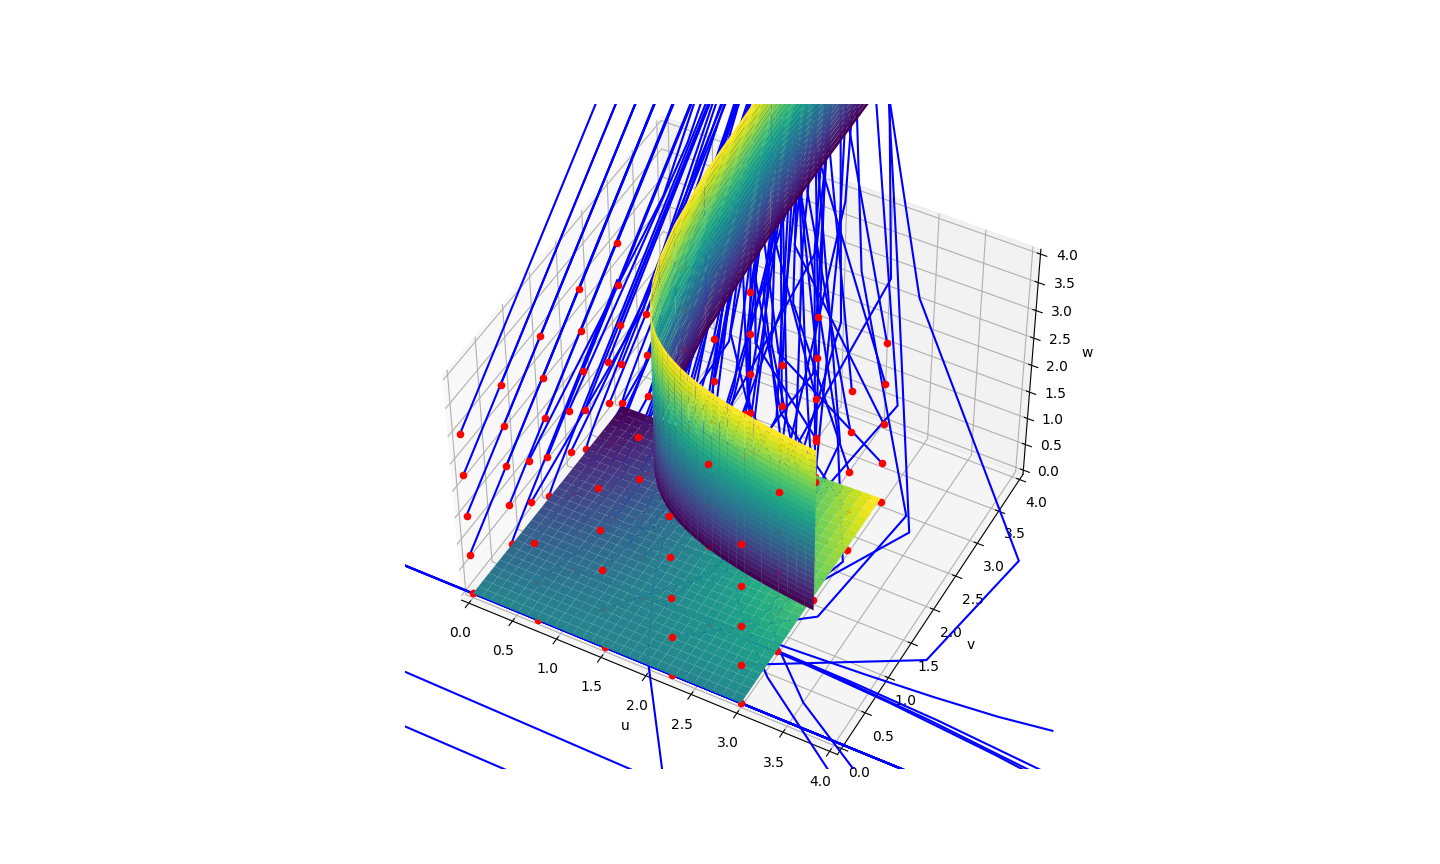
\includegraphics[width=1\textwidth]{Figure_11.png}\\

Видим, что траектории с \(\w>0\) удаляются от неподвижных точек.\\

Так как обе неподвижные точки находятся на плоскости \(w=0\), рассмотрим поведение траекторий, находящихся на данной плоскости.\\

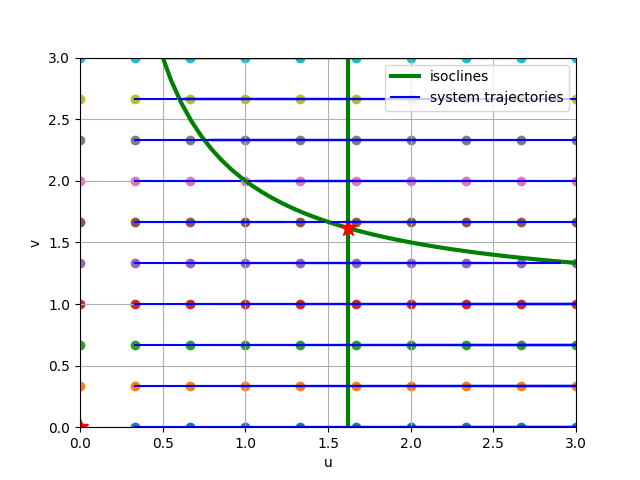
\includegraphics[width=1\textwidth]{Figure_13.png}\\

Из графика (а также из того факта, что при \(w=0\)  \(u' = 0\)) получаем горизонтально направленные траектории, из чего следует, что не существует траекторий, которые попали бы из точки \(\overline{O}\) в точку \(\overline{P}\), поскольку для этого было бы необходимо иметь \(u' > 0\).\\

Получаем, что в данной системе нет волновых решений.


\newpage
\clearpage
\begin{thebibliography}{0}
\addcontentsline{toc}{section}{Список литературы}
	\bibitem{OC_lect}Братусь~А.\,С., Новожилов~А.\,С., Платонов~А.\,П. \label{Bratus_book}
	\emph{Динамические системы и модели биологии},
	2011 г.
\end{thebibliography}
\end{document}